\addcontentsline{toc}{chapter}{Glossary}
\chapter*{Glossary\markboth{Glossary}{}}

\begin{hangparas}{.25in}{1}
	\label{akathist}
	\gloss{akathist}{A series of hymns consisting of thirteen kontakia (short hymns), each followed by a refrain, and the first twelve followed also by an \textit{oikos} (pl. textit{oikoi}) (an intoned or chanted hymn).}
	
	\label{hegumen}
	\gloss{hegumen}{An abbot, a superior of a monastic establishment.}
	
	\label{hierodeacon}
	\gloss{hierodeacon}{A monk who has been ordained to the diaconate.}
	
	\label{hieromonk}
	\gloss{hieromonk}{A monk who has been ordained to the priesthood.}
	
	\label{hiero-schemamonk}
	\gloss{hiero-schemamonk}{A schemamonk (see below) who has been ordained to the priesthood.}
	
	\label{litya}
	\gloss{litya}{(Gk. \textit{liti}) Literally, ''Entreaty.'' A special service of supplication chanted during Great Vespers, usually in the narthex of the church.}
	
	\label{mantia}
	\gloss{mantia}{(Gk. \textit{mandias}) The outer garment of a monk, a wide garment, very long, and without sleeves, worn as a cape over his other monastic garments. This is given at the tonsure of a rassophor monk into the lesser schema, at which one pronounces vows and becomes a monk proper. Hence, to be tonsured into the mantia is to become a full-fledged monk.}
	
	\label{moleben}
	\gloss{moleben}{A special service of prayers of thanksgiving and petition offered on the occasion of some special occurrence in the life of an individual or of the nation. A \textit{moleben} may be requested at a time of special need or at a time of special thanksgiving. Somewhat equivalent to the \textit{Paraclesis}.}
	
	\label{nabedrennik}
	\gloss{nabedrennik}{A rectangular article of the priest's vestments, suspended by a shoulder strap, worn at the side hanging down from the waist. This article is bestowed by a bishop as an ecclesiastical dignity. It is not to be confused with the diamond shaped \textit{palitsa}, which may be given subsequently. This latter corresponds to the Greek \textit{epigonation}.}
	
	\label{pannikhida}
	\gloss{pannikhida}{A special service of prayers offered on behalf of the faithful who have reposed. At the service a dish of boiled wheat or rice with honey is set forth. A \textit{pannikhida} may be offered in conjunction with the Divine Liturgy or may form a separate service. This may be offered in church or at the grave of the reposed.}
	
	\label{paraman}
	\gloss{paraman}{The name derives from the Greek \textit{paramandias} meaning ``something besides, or added to the mantia.'' This is a square of material on which is depicted the Cross of Christ with the lance and reed and the inscription. ``I wear upon my body the wounds of my Lord.'' By means of cords or ribbons tied to each corner it is fastened around the shoulders and waist of the monk. This is given to monastics at the tonsure into the mantia.}
	
	\label{Philokalia}
	\gloss{Philokalia}{A compilation of exalted texts on prayer and the spiritual life which span from the fourth to the fifteenth centuries, compiled by SS. Macarios of Corinth and Nicodemos of the Holy Mountain, first printed in 1792. An abridged translation into Russian, the \textit{Dobrotolyubie}, by St. Paissy Velichkovsky, appeared in 1793. In the Elder Joseph's own days the edition of Theofan the Recluse appeared, considerably longer than the original, some 3,000 pages in all.}
	
	\label{prosphora}
	\gloss{prosphora}{The specially-prepared bread stamped with the Eucharistic Seal which is brought by the faithful to church to be used at the preparation of the Holy Eucharist. The faithful submit with the prosphora names of the living and the reposed to be commemorated at the preparation. The priest, having commemorated the names and having removed portions, placing them on the holy paten, returns the remainder of the prosphora to the one who submitted it. Prosphora so used may also be kept and distributed afterwards as a blessing from the Divine Liturgy.}
	
	\label{rassophor}
	\gloss{rassophor}{The name derives from the rassa, the robe with wide sleeves, and means ``wearer of the rassa.'' A rassophor monk has been tonsured into the monastic estate, but as yet has pronounced no vows.}
	
	\label{schema}
	\gloss{schema}{A piece of material decorated with many crosses and inscriptions, also called the \textit{analavon}, worn by monks tonsured into the highest state of monastics.}
	
	\label{schemamonk}
	\gloss{schemamonk}{The highest state of monastics, a monk tonsured into the great schema takes vows of complete renunciation of the world. In place of the \textit{paraman} he wears the \textit{analavon}, or schema, which is ornamented with many crosses and worn suspended from the shoulders.}
	
	\label{Typicon}
	\gloss{Typicon}{The book that contains the rule or order for the daily offices chanted in church. In the monastic context, it signifies also the Rule adhered to by a monastic community.}
\end{hangparas}

\bigpicgeometry
\vspace*{\fill}
\thispagestyle{empty}
\newsavebox{\map}
\begin{figure}[ht]
\center
  \savebox{\map}{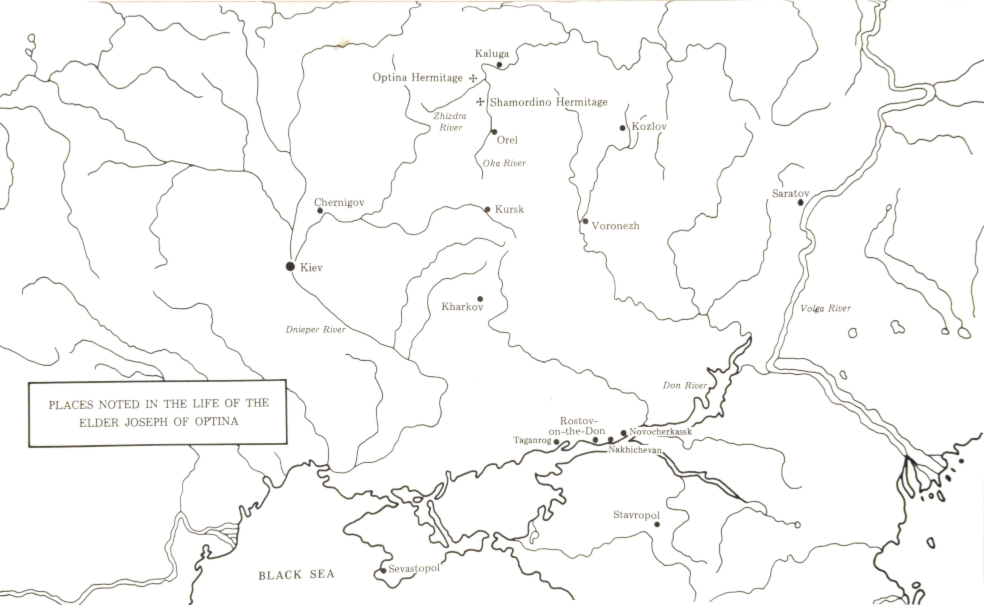
\includegraphics[width=8.5in]{Images/Optina_Map.png}}% Image to be included}
  \rotatebox{90}{% Rotate 90 CCW
    \begin{minipage}{\wd\map}
      \usebox{\map}
    \end{minipage}}
\end{figure}
\vspace*{\fill}\restoregeometry